% Provenance (never printed): cycle 2 "Questionner le monde de la matiere"
% (solid materials, observing and sorting) and cycle 3 theme 4 (local geology,
% rocks for building); see sources/book1/PROVENANCE.md. Book 1, grade 3, ch. 1.
\chapter{الحجارة والحصى والرمل}\label{ch:g3:stones-pebbles-sand}

توم في عطلة قرب \omterm{def:g1:landscapes-around-us:water}{نهر}. على الضفة المكسوة \omterm{def:g3:stones-pebbles-sand:pebble}{بالحصى}، حيث الماء ضحل، يلتقط
\omterm{def:g3:stones-pebbles-sand:pebble}{حصاة}. إنها ملساء مستديرة، تكاد تشبه البيضة، وتملأ كفه. وفي الأسبوع
الماضي، وهو يمشي مع والديه على درب جبلي في أعالي \omterm{def:g1:landscapes-around-us:landform}{الوادي} نفسه، رأى حجارة
لها اللون نفسه ملقاة تحت منحدر صخري --- لكن تلك الحجارة كانت حادة، لها
حواف وزوايا.

كيف صار حجر حاد من \omterm{def:g1:landscapes-around-us:landform}{الجبل} \omterm{def:g3:stones-pebbles-sand:pebble}{حصاة} ملساء مستديرة في أسفل \omterm{def:g1:landscapes-around-us:landform}{الوادي}؟ لنعرف ذلك،
لنبدأ \omterm{def:g3:stones-pebbles-sand:rock}{بالصخر} نفسه.

\begin{omfigure}
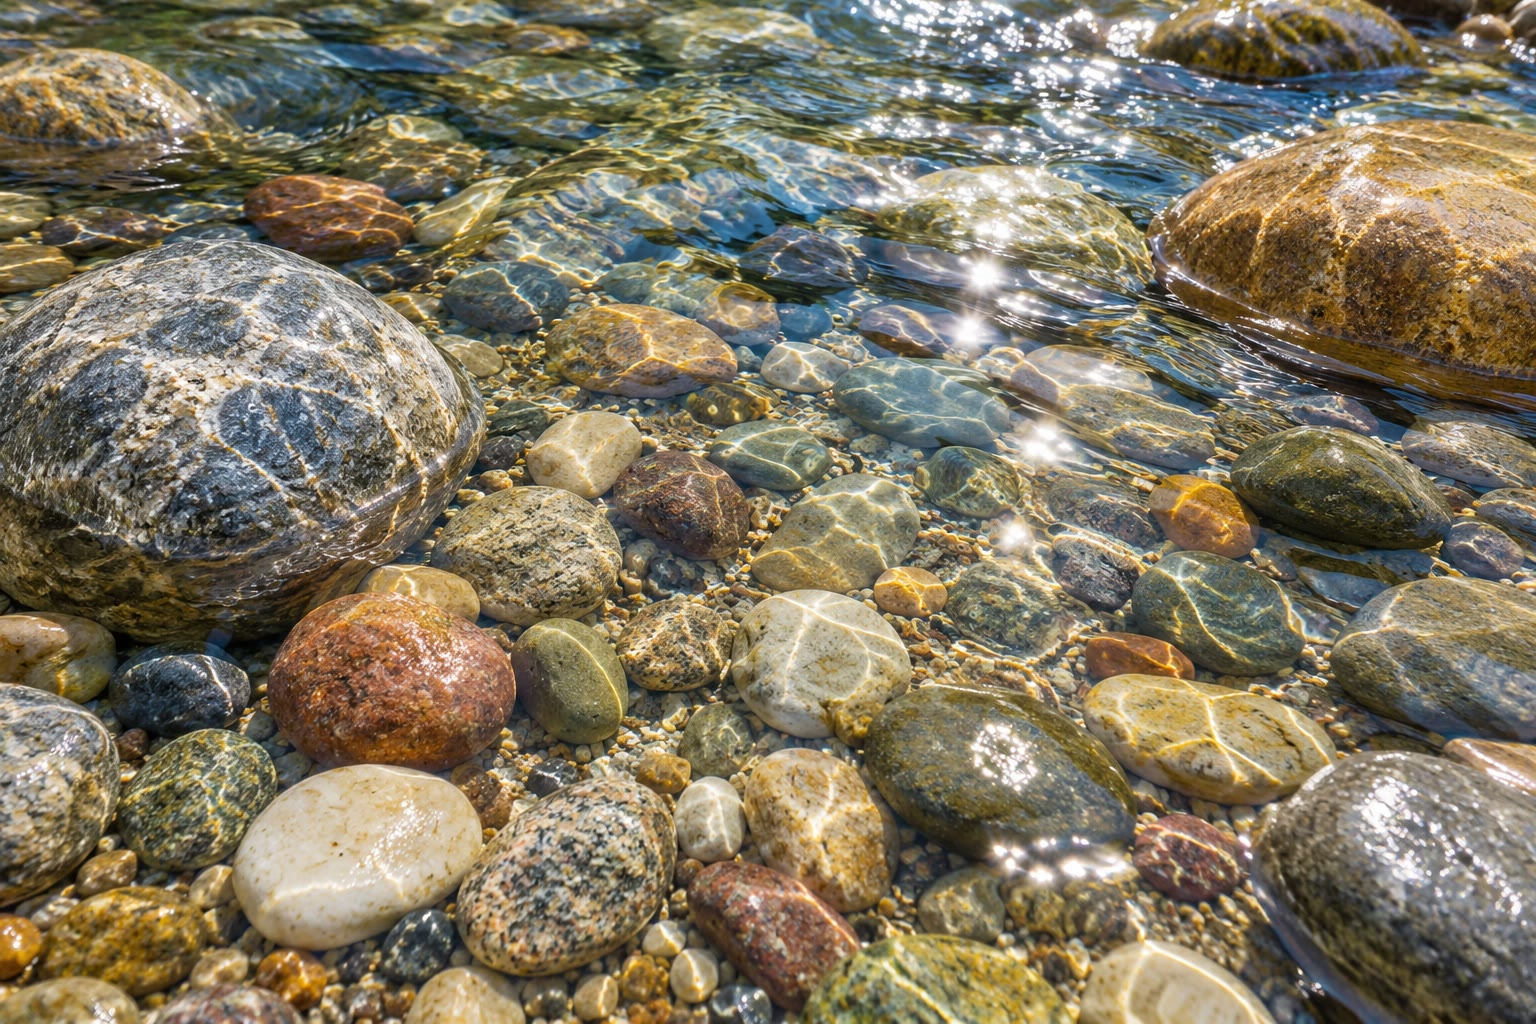
\includegraphics[width=0.62\linewidth]{images/book1/ai/g3-stream-pebbles.jpg}

{\small \omterm{def:g3:stones-pebbles-sand:pebble}{حصى} مستدير تحت ماء جدول صافٍ.}
\end{omfigure}

\begin{recall}
في \omterm{def:g1:landscapes-around-us:landscape}{المنظر} \omterm{def:g1:landscapes-around-us:landform}{جبال} \omterm{def:g1:landscapes-around-us:landform}{وتلال} \omterm{def:g1:landscapes-around-us:landform}{وأودية} \omterm{def:g1:landscapes-around-us:landform}{وسهول}، \omterm{def:g1:landscapes-around-us:water}{وأنهار} تجري من الأرض العالية نزولًا
إلى \omterm{def:g2:water-on-earth:ocean}{البحر} (\cref{ch:g1:landscapes-around-us}). والطبقة العليا من الأرض،
حيث تنمو النباتات، هي التربة: وكتب الأحياء تحكي كيف تصنعها الكائنات
الحية.
\end{recall}

\section{الصخر: الأرض الصلبة تحت أقدامنا}

احفر حفرة عميقة في حديقة. ستجد أولًا تربة داكنة لينة فيها جذور. وتحتها
تصير التربة أفتح لونًا وأكثر حجارة. ولو استطعت أن تحفر عميقًا بما يكفي،
لوصلت دائمًا إلى شيء صلب لا تقطعه المجرفة:
\omterm{def:g3:stones-pebbles-sand:rock}{الصخر}.

\begin{definition}[الصخر والصخر الأساسي]\label{def:g3:stones-pebbles-sand:rock}
\emph{الصخر}\index{صخر} مادة طبيعية صلبة تتكون منها الأرض الصلبة.
و\emph{الصخر الأساسي}\index{صخر أساسي} هو الصخر الصلب الذي يمتد تحت
التربة في كل مكان على اليابسة، وتحت \omterm{def:g3:stones-pebbles-sand:sand}{رمل} قاع \omterm{def:g2:water-on-earth:ocean}{البحر}
ووحله.
\end{definition}

في أكثر الأماكن تخفي التربةُ والعشب والأشجار الصخرَ الأساسي. ونراه حيث لا
توجد تربة تغطيه: في سفوح \omterm{def:g1:landscapes-around-us:landform}{الجبال} الشديدة الانحدار، وفي الجروف على
شاطئ \omterm{def:g2:water-on-earth:ocean}{البحر}، وعلى جوانب الطرق التي شُقت عبر
\omterm{def:g1:landscapes-around-us:landform}{تلة}.

\begin{omfigure}
\begin{tikzpicture}[x=1cm, y=1cm, font=\small]
  % bedrock
  \fill[omLithGranite!60] (0,0) rectangle (11,2.2);
  \foreach \x/\y in {0.6/0.5, 1.8/1.4, 3.1/0.7, 4.4/1.6, 5.6/0.4, 6.9/1.2, 8.3/0.6, 9.6/1.5, 10.3/0.4}
    \draw[black!40, line width=0.4pt] (\x,\y) -- ++(0.5,0.25);
  % soil (thick on the left, missing on the steep right)
  \fill[brown!55] (0,2.2) -- (0,3.4) .. controls (2,3.5) and (4,3.4) .. (5.6,3.2) -- (6.4,2.9) -- (6.4,2.2) -- cycle;
  \fill[brown!30] (0,2.2) rectangle (6.4,2.65);
  % rock showing on the right: a hill side with no soil
  \fill[omLithGranite!60] (6.4,2.2) -- (6.4,2.9) -- (7.6,3.9) -- (8.8,4.3) -- (11,4.3) -- (11,2.2) -- cycle;
  \draw[black!60] (0,3.4) .. controls (2,3.5) and (4,3.4) .. (5.6,3.2) -- (6.4,2.9) -- (7.6,3.9) -- (8.8,4.3) -- (11,4.3);
  % grass and roots
  \foreach \x in {0.3,0.8,...,5.3}
    \draw[green!50!black, line width=0.6pt] (\x,{3.4-0.04*\x}) -- ++(0.05,0.18);
  \foreach \x in {1.2,3.4,4.9}
    \draw[brown!80!black, line width=0.5pt] (\x,3.3) -- ++(-0.1,-0.5) -- ++(0.15,-0.3);
  % labels
  \node[anchor=west] at (11.2,3.6) {صخر يظهر};
  \node[anchor=west] at (11.2,3.2) {على السطح};
  \draw[black!60] (11.15,3.4) -- (9.6,4.15);
  \node[anchor=east] at (-0.2,2.9) {التربة};
  \draw[black!60] (-0.15,2.9) -- (0.6,2.9);
  \node[anchor=west] at (11.2,1.1) {الصخر الأساسي};
  \draw[black!60] (11.15,1.1) -- (10.6,1.1);
\end{tikzpicture}

{\small مقطع في الأرض. تحت التربة يوجد دائمًا \omterm{def:g3:stones-pebbles-sand:rock}{الصخر الأساسي} الصلب. وعلى
سفح \omterm{def:g1:landscapes-around-us:landform}{التلة} الشديد الانحدار، على اليمين، لا توجد تربة فيظهر \omterm{def:g3:stones-pebbles-sand:rock}{الصخر} على
السطح.}
\label{fig:g3:stones-pebbles-sand:ground}
\end{omfigure}

\section{من الصخر إلى الحصى}

\omterm{def:g3:stones-pebbles-sand:rock}{الصخر} صلب، لكنه لا يدوم إلى الأبد. ففي الشتاء يدخل الماء في شقوق \omterm{def:g3:stones-pebbles-sand:rock}{الصخر}،
ويتجمد فيتمدد، ويدفع الشقوق فيوسعها. والجذور أيضًا تنمو في الشقوق.
وشيئًا فشيئًا تنفصل قطع وتسقط: من هنا تأتي الحجارة الحادة التي تحت
منحدرات \omterm{def:g1:landscapes-around-us:landform}{الجبال}.

حين يسقط حجر حاد في جدول جبلي، يدحرجه الماء على القاع، ويصدمه بحجارة
أخرى، ويجره فوق \omterm{def:g3:stones-pebbles-sand:sand}{الرمل}. وزواياه هي أول ما يُبرى منه. وكلما ابتعد في
رحلته صار أكثر استدارة وملاسة. وحين يصل إلى أسفل \omterm{def:g1:landscapes-around-us:landform}{الوادي} يكون قد صار
\omterm{def:g3:stones-pebbles-sand:pebble}{حصاة}.

\begin{definition}[الحصاة والحصباء]\label{def:g3:stones-pebbles-sand:pebble}
\emph{الحصاة}\index{حصاة} قطعة صغيرة من \omterm{def:g3:stones-pebbles-sand:rock}{الصخر} جعلها الماء مستديرة ملساء
وهو يدحرجها، في \omterm{def:g1:landscapes-around-us:water}{نهر} أو على شاطئ.
و\emph{الحصباء}\index{حصباء} كتلة من الحجارة الصغيرة والحصى المتجمعة
معًا، حبيباتها أكبر من حبيبات \omterm{def:g3:stones-pebbles-sand:sand}{الرمل}.
\end{definition}

\begin{omfigure}
\begin{tikzpicture}[x=1cm, y=1cm, font=\small]
  \draw[ocBlue!70!black, line width=1.2pt, -{Stealth[length=3mm]}] (0,0) -- (12.2,0);
  \node[below, font=\scriptsize] at (6.1,-0.15) {الجدول يحمل الحجر نزولًا، أبعد قليلًا مع كل فيضان};
  \foreach \x/\shape/\t in {
     0.8/{(-0.55,-0.1) -- (-0.2,0.5) -- (0.35,0.55) -- (0.6,0.05) -- (0.3,-0.45) -- (-0.35,-0.5) -- cycle}/سقط من الصخر,
     4.0/{(-0.5,-0.1) [rounded corners=4pt] -- (-0.2,0.45) -- (0.3,0.5) -- (0.55,0.05) -- (0.3,-0.4) -- (-0.35,-0.45) -- cycle}/بُريت زواياه,
     7.2/{(-0.45,-0.05) [rounded corners=8pt] -- (-0.15,0.42) -- (0.3,0.45) -- (0.5,0.05) -- (0.3,-0.35) -- (-0.3,-0.4) -- cycle}/أكثر استدارة وأصغر,
     10.4/{(0,0) ellipse (0.45 and 0.3)}/حصاة ملساء} {
    \begin{scope}[shift={(\x,1.1)}]
      \fill[omLithGranite!80, draw=black!70] \shape;
    \end{scope}
    \node[font=\scriptsize] at (\x,0.35) {\t};
  }
\end{tikzpicture}

{\small رحلة حجر في \omterm{def:g1:landscapes-around-us:water}{نهر}: حاد حين يسقط من \omterm{def:g3:stones-pebbles-sand:rock}{الصخر}، ومستدير أملس بعد رحلة
طويلة مع التيار.}
\label{fig:g3:stones-pebbles-sand:journey}
\end{omfigure}

\begin{remark}[نقرأ شكل الحجر]\label{rem:g3:stones-pebbles-sand:shape}
شكل الحجر يحكي لنا قصته. فالحجر الحاد لم يبتعد كثيرًا عن \omterm{def:g3:stones-pebbles-sand:rock}{الصخر} الذي
انفصل عنه. \omterm{def:g3:stones-pebbles-sand:pebble}{والحصاة} المستديرة الملساء دحرجها الماء زمنًا طويلًا، في \omterm{def:g1:landscapes-around-us:water}{نهر}
أو بفعل أمواج \omterm{def:g2:water-on-earth:ocean}{البحر}.
\end{remark}

\section{الرمل والوحل}

الحجارة \omterm{def:g3:stones-pebbles-sand:pebble}{والحصى} التي يصطدم بعضها ببعض تكسر منها أيضًا قطعًا صغيرة جدًا.
وعلى مدى زمن طويل جدًا تصير هذه القطع الصغيرة \omterm{def:g3:stones-pebbles-sand:sand}{رملًا}. انظر إلى \omterm{def:g3:stones-pebbles-sand:sand}{الرمل} من
خلال عدسة مكبرة: كل حبة قطعة صغيرة من \omterm{def:g3:stones-pebbles-sand:rock}{صخر}، أو من صدفة، ومستديرة في
الغالب هي أيضًا.

\begin{definition}[الرمل والوحل]\label{def:g3:stones-pebbles-sand:sand}
% ledger: usgs:wentworth
\emph{الرمل}\index{رمل} يتكون من حبيبات مفككة من \omterm{def:g3:stones-pebbles-sand:rock}{صخر} مكسور يقل قطرها
عن 2 مليمتر: لا نزال نرى كل حبة. و\emph{الوحل}\index{وحل} يتكون من
حبيبات صغيرة جدًا حتى إننا لا نراها واحدة واحدة؛ وهو إذا ابتل لين
لزج.
\end{definition}

يفرز الجيولوجيون قطع \omterm{def:g3:stones-pebbles-sand:rock}{الصخر} المكسور بحسب حجمها، من الأكبر إلى الأصغر:
الجلاميد، ثم \omterm{def:g3:stones-pebbles-sand:pebble}{الحصى} \omterm{def:g3:stones-pebbles-sand:pebble}{والحصباء}، ثم \omterm{def:g3:stones-pebbles-sand:sand}{الرمل}، ثم \omterm{def:g3:stones-pebbles-sand:sand}{الوحل}.

\begin{omfigure}
\begin{tikzpicture}[x=1mm, y=1mm, font=\small]
  % true size: 1 unit = 1 mm
  \draw[black!40] (0,-14) -- (150,-14);
  \foreach \x in {0,10,...,150} \draw[black!40] (\x,-14) -- (\x,-12.5);
  \foreach \x in {0,50,100,150} \node[font=\scriptsize, below] at (\x,-14.5) {\pgfmathparse{int(\x/10)}\pgfmathresult\,cm};
  % mud: too small
  \node[font=\scriptsize, align=center] at (6,14) {وحل};
  \fill[brown!60] (6,0) circle (0.05);
  \node[font=\scriptsize, align=center] at (6,4.5) {حبيبات أصغر\\من أن تُرى};
  % sand grains: up to 2 mm
  \node[font=\scriptsize] at (28,14) {رمل};
  \foreach \x/\r in {22/0.3, 25/0.5, 28/0.75, 32/1.0}
    \fill[yellow!60!brown, draw=black!50, line width=0.2pt] (\x,0) circle (\r);
  \node[font=\scriptsize, align=center] at (28,5) {\foreignlanguage{arabic}{أصغر من}\\\foreignlanguage{arabic}{\babelsublr{2} مليمتر}};
  % gravel and pebbles
  \node[font=\scriptsize] at (78,22) {حصباء وحصى};
  \fill[omLithGranite!80, draw=black!60] (52,0) ellipse (2 and 1.5);
  \fill[black!25, draw=black!60] (62,0) ellipse (4 and 3);
  \fill[omLithGranite!80, draw=black!60] (78,0) ellipse (8 and 6);
  \fill[black!30, draw=black!60] (104,0) ellipse (15 and 10);
  % boulder: off scale
  \node[font=\scriptsize] at (138,22) {جلمود};
  \fill[black!20, draw=black!60] (128,-10) .. controls (127,8) and (135,16) .. (142,15) .. controls (150,14) and (152,4) .. (149,-10) -- cycle;
  \node[font=\scriptsize, align=center, fill=white, fill opacity=0.7, text opacity=1, inner sep=1pt] at (139,4) {مرسوم أصغر\\بكثير};
\end{tikzpicture}

{\small حبيبات \omterm{def:g3:stones-pebbles-sand:rock}{الصخر} المكسور من الأصغر إلى الأكبر. \omterm{def:g3:stones-pebbles-sand:sand}{الوحل} \omterm{def:g3:stones-pebbles-sand:sand}{والرمل} \omterm{def:g3:stones-pebbles-sand:pebble}{والحصباء}
\omterm{def:g3:stones-pebbles-sand:pebble}{والحصى} مرسومة بحجمها الحقيقي: قارن بمسطرة. وقد يكون الجلمود بحجم كرسي،
أو بحجم بيت.}
\label{fig:g3:stones-pebbles-sand:sizes}
\end{omfigure}

\begin{omfigure}
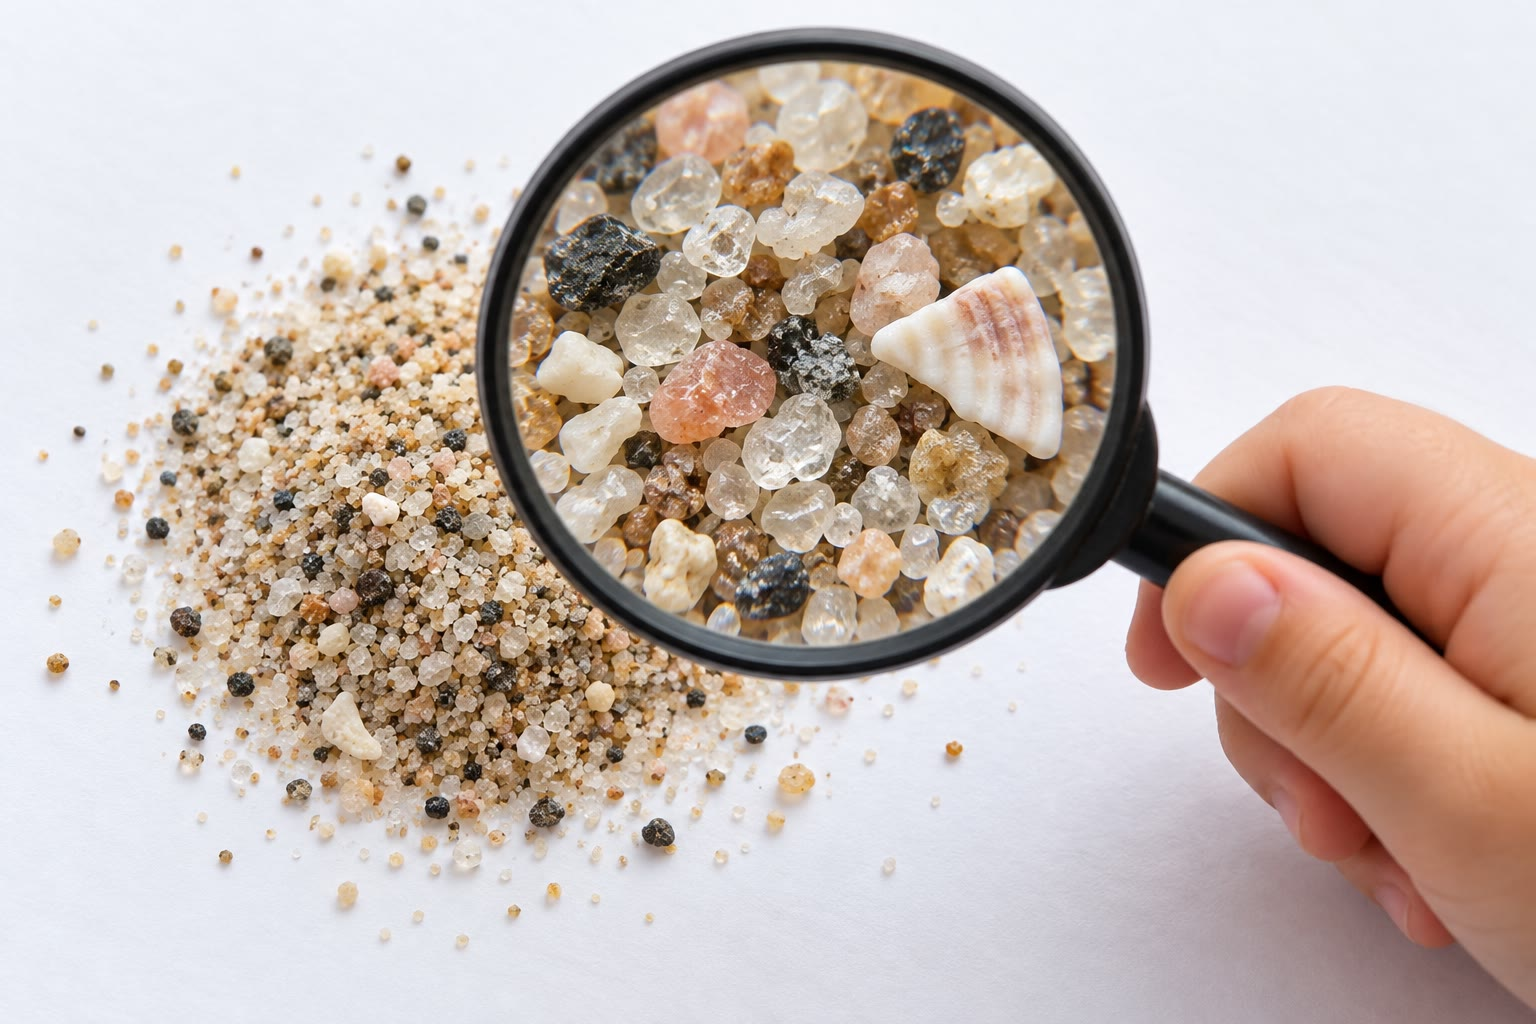
\includegraphics[width=0.55\linewidth]{images/book1/ai/g3-sand-magnifier.jpg}

{\small \omterm{def:g3:stones-pebbles-sand:sand}{رمل} الشاطئ من خلال عدسة مكبرة: حبيبات صغيرة جدًا من \omterm{def:g3:stones-pebbles-sand:rock}{الصخر} وقطع
من الصدف.}
\end{omfigure}

\begin{method}[فرز الصخر المكسور بحسب الحجم]\label{met:g3:stones-pebbles-sand:sort}
لتسمية قطعة من \omterm{def:g3:stones-pebbles-sand:rock}{الصخر} المكسور، انظر إلى حجمها:
\begin{enumerate}
  \item إذا لم تستطع أن ترى الحبيبات، حتى عن قرب، فهو \omterm{def:g3:stones-pebbles-sand:sand}{وحل}؛
  \item إذا استطعت أن ترى كل حبة، لكن كل واحدة أصغر من 2
        مليمتر (سمك قطعة نقدية)، فهو \omterm{def:g3:stones-pebbles-sand:sand}{رمل}؛
  \item إذا كانت القطع أكبر من ذلك، لكنك تستطيع أن تمسك واحدة منها في
        يدك، فهي \omterm{def:g3:stones-pebbles-sand:pebble}{حصباء} \omterm{def:g3:stones-pebbles-sand:pebble}{وحصى}؛
  \item إذا كانت القطعة أثقل من أن تُرفع، فهي جلمود.
\end{enumerate}
\end{method}

\begin{example}[أين نجد كل حجم؟]\label{ex:g3:stones-pebbles-sand:where}
الماء السريع يستطيع أن يحمل حجارة كبيرة؛ والماء البطيء يتركها ولا يحمل إلا
الحبيبات الصغيرة. لذلك توجد الجلاميد والحجارة الحادة في الجداول الجبلية
الشديدة الانحدار؛ \omterm{def:g3:stones-pebbles-sand:pebble}{والحصى} \omterm{def:g3:stones-pebbles-sand:pebble}{والحصباء} على ضفاف \omterm{def:g1:landscapes-around-us:water}{النهر} في \omterm{def:g1:landscapes-around-us:landform}{الوادي}؛ ويتجمع \omterm{def:g3:stones-pebbles-sand:sand}{الرمل}
على الشواطئ وفي منعطفات \omterm{def:g1:landscapes-around-us:water}{النهر} الهادئة؛ ويترسب \omterm{def:g3:stones-pebbles-sand:sand}{الوحل} حيث يكاد الماء يسكن،
في البرك \omterm{def:g1:landscapes-around-us:water}{والبحيرات} ومصبات \omterm{def:g1:landscapes-around-us:water}{الأنهار}.
\end{example}

\section{صخور صلبة وصخور لينة}

ليست \omterm{def:g3:stones-pebbles-sand:rock}{الصخور} كلها صلبة بالقدر نفسه. فبعضها، مثل الغرانيت، صلب حتى إنه يخدش
الزجاج ويبقى آلاف السنين في جدار. وبعضها يتفتت في اليد، مثل الطباشير، الذي
يترك أثرًا أبيض على السبورة. وبعض \omterm{def:g3:stones-pebbles-sand:rock}{الصخور} يتكون من حبيبات نراها؛ وبعضها
أملس يبدو متشابهًا من جهة إلى أخرى.

\begin{example}[مقارنة ثلاثة صخور]\label{ex:g3:stones-pebbles-sand:three}
\emph{الغرانيت} مرقط بحبيبات وردية وبيضاء وسوداء، وهو صلب جدًا.
و\emph{الحجر الرملي} يتكون من حبيبات \omterm{def:g3:stones-pebbles-sand:sand}{رمل} ملتصقة معًا؛ وإذا فركته بإصبعك
أفلت منه أحيانًا بضع حبيبات. و\emph{الطباشير} أبيض لين يتحول مسحوقًا.
وستتعلم في سنة لاحقة كيف تكوّن كل واحد
منها.
\end{example}

\begin{omfigure}
\begin{tikzpicture}[font=\small]
  % three stones seen through a magnifying glass (drawn, not to scale)
  % granite: interlocking grains of three colours
  \begin{scope}
    \clip (0,0) circle (1.5);
    % a jittered lattice: the cells tile the disk with no gap, like the
    % interlocking crystals of granite
    \foreach \i in {-6,...,5} \foreach \j in {-6,...,5} {
      \pgfmathtruncatemacro{\c}{mod(abs(37*\i+17*\j+\i*\j),7)}
      \ifcase\c \def\col{pink!70}\or\def\col{pink!45}\or\def\col{white}\or
        \def\col{black!12}\or\def\col{white}\or\def\col{black!80}\else\def\col{pink!60}\fi
      \fill[\col, draw=black!35, line width=0.3pt]
        ({0.27*\i+0.07*sin(90*\i+131*\j)},{0.27*\j+0.07*cos(77*\i+61*\j)}) --
        ({0.27*(\i+1)+0.07*sin(90*(\i+1)+131*\j)},{0.27*\j+0.07*cos(77*(\i+1)+61*\j)}) --
        ({0.27*(\i+1)+0.07*sin(90*(\i+1)+131*(\j+1))},{0.27*(\j+1)+0.07*cos(77*(\i+1)+61*(\j+1))}) --
        ({0.27*\i+0.07*sin(90*\i+131*(\j+1))},{0.27*(\j+1)+0.07*cos(77*\i+61*(\j+1))}) -- cycle;
    }
  \end{scope}
  \draw[black!70, line width=2pt] (0,0) circle (1.5);
  \node at (0,-1.9) {غرانيت};
  \node[font=\scriptsize, align=center] at (0,-2.45) {حبيبات كبيرة بثلاثة\\ألوان، متشابكة};
  % sandstone: rounded grains touching
  \begin{scope}[xshift=4.2cm]
    \clip (0,0) circle (1.5);
    \fill[brown!45] (-1.6,-1.6) rectangle (1.6,1.6);
    \foreach \x in {-1.5,-1.1,...,1.6} \foreach \y in {-1.5,-1.15,...,1.6}
      \fill[yellow!50!brown!70, draw=brown!70!black, line width=0.3pt]
        ({\x+0.08*sin(97*\x+61*\y)},{\y+0.07*cos(53*\x-89*\y)}) circle ({0.16+0.03*sin(71*\x*\y)});
  \end{scope}
  \draw[black!70, line width=2pt] (4.2,0) circle (1.5);
  \node at (4.2,-1.9) {حجر رملي};
  \node[font=\scriptsize, align=center] at (4.2,-2.45) {حبيبات رمل مستديرة\\ملتصقة معًا};
  % chalk: smooth, no grains to see
  \begin{scope}[xshift=8.4cm]
    \fill[white] (0,0) circle (1.5);
  \end{scope}
  \draw[black!70, line width=2pt] (8.4,0) circle (1.5);
  \node at (8.4,-1.9) {طباشير};
  \node[font=\scriptsize, align=center] at (8.4,-2.45) {أبيض أملس: حبيباته\\أصغر من أن تُرى};
\end{tikzpicture}

{\small ثلاثة \omterm{def:g3:stones-pebbles-sand:rock}{صخور} من خلال عدسة مكبرة (رسم). حبيبات الغرانيت والحجر الرملي
تُرى؛ والطباشير يبدو متشابهًا في كل مكان.}
\label{fig:g3:stones-pebbles-sand:magnified}
\end{omfigure}

\begin{method}[النظر إلى حجر عن قرب]\label{met:g3:stones-pebbles-sand:look}
لوصف حجر، انظر إليه والمسه، دون أن تكسره:
\begin{enumerate}
  \item لونه، أو ألوانه؛
  \item شكله: حاد له زوايا، أم مستدير أملس؛
  \item حبيباته: هل تراها؟ هل هي كلها متشابهة، أم بألوان
        مختلفة؟
  \item ملمسه: صلب، أم لين يترك أثرًا على الورق؟
\end{enumerate}
اكتب ما تراه في جدول، سطرًا لكل حجر.
\end{method}

\begin{example}[جدول لثلاثة حجارة]\label{ex:g3:stones-pebbles-sand:table}
تصف ميا ثلاثة حجارة من صندوق في المدرسة.
\begin{center}\small
\begin{tabular}{llll}
\hline
الحجر & اللون & الشكل & الحبيبات \\
\hline
أ & وردي وأبيض وأسود & مستدير & كبيرة، ثلاثة ألوان \\
ب & بني مصفر & حاد & صغيرة، متشابهة \\
ج & أبيض & حاد & لا تُرى \\
\hline
\end{tabular}
\end{center}
والحجر ج يترك أيضًا أثرًا أبيض على الورق. وحسب المثال السابق، يشبه الحجر أ
الغرانيت، والحجر ب الحجر الرملي، والحجر ج الطباشير. والحجر أ مستدير: لقد
دحرجه الماء زمنًا طويلًا.
\end{example}

\section{الحجارة التي نبني بها}

منذ آلاف السنين يبني الناس \omterm{def:g3:stones-pebbles-sand:rock}{بالصخر} الذي حولهم. وفي القرى القديمة لمنطقة ما،
تكون الجدران في الغالب كلها بلون واحد، لأنها بُنيت بحجر أقرب
\omterm{def:g1:landscapes-around-us:landform}{تلة}.

\begin{definition}[حجر البناء]\label{def:g3:stones-pebbles-sand:building-stone}
\emph{حجر البناء}\index{حجر البناء} \omterm{def:g3:stones-pebbles-sand:rock}{صخر} يُقطع أو يُشكَّل لبناء الجدران
أو السطوح أو الدرج أو الجسور أو الأرصفة.
\end{definition}

لكل \omterm{def:g3:stones-pebbles-sand:rock}{صخر} فائدة. فالغرانيت الصلب يصنع جدرانًا ودرجات وحواف أرصفة تدوم
قرونًا. وبعض \omterm{def:g3:stones-pebbles-sand:rock}{الصخور}، مثل الأردواز، ينفلق صفائح رقيقة مسطحة: إذا وُضعت
بعضها فوق بعض صنعت سطوحًا تمنع المطر. والحجر الرملي والحجر الجيري
لينان بما يكفي لقطعهما كتلًا منتظمة.

\begin{omfigure}
\begin{minipage}[b]{0.49\linewidth}\centering
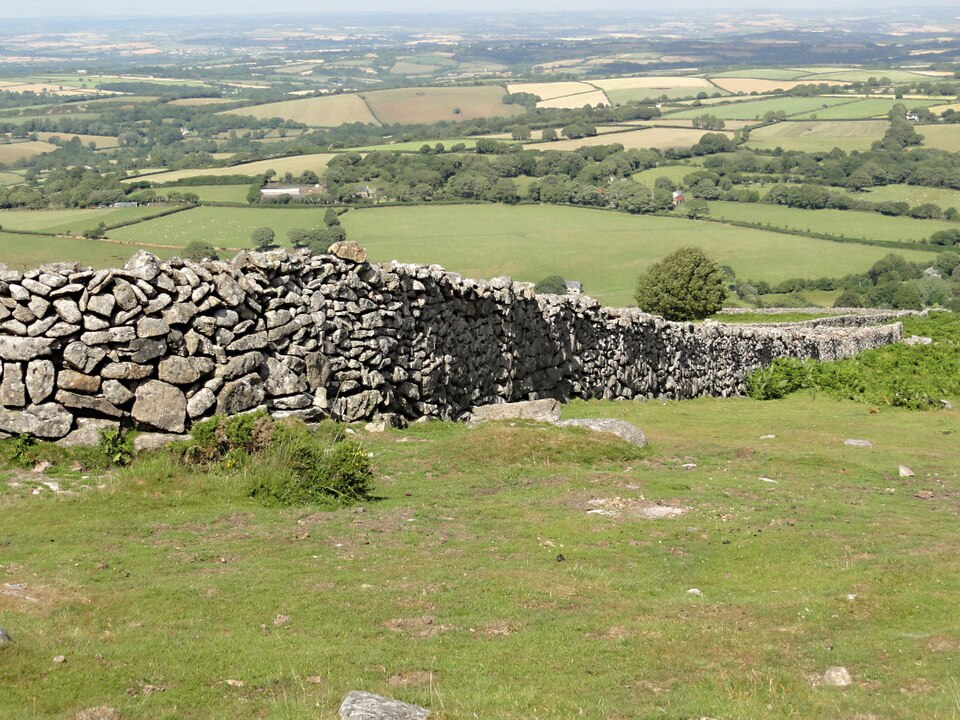
\includegraphics[width=\linewidth]{images/book1/g3-granite-wall.jpg}

{\small جدار من كتل الغرانيت، بُني بلا ملاط. الصورة: توني
أتكن، موقع جيوغراف (CC BY-SA 2.0).}
\end{minipage}\hfill
\begin{minipage}[b]{0.49\linewidth}\centering
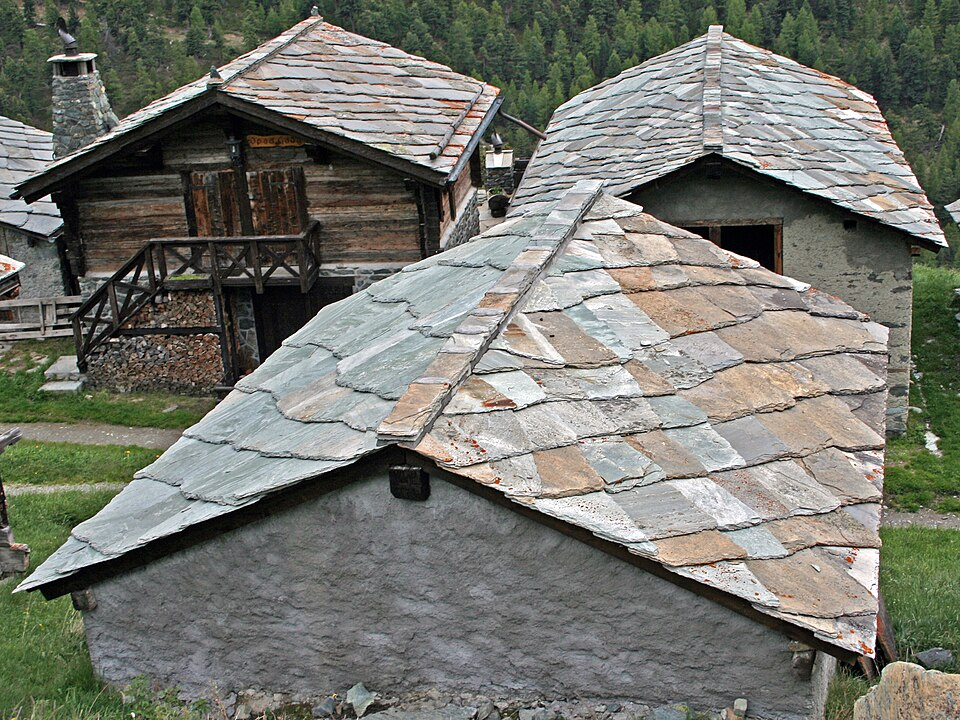
\includegraphics[width=\linewidth]{images/book1/g3-slate-roof.jpg}

{\small سطوح من ألواح حجرية رقيقة مسطحة في قرية جبلية في
سويسرا. الصورة: مايكل سي. رايغل (CC BY-SA 3.0).}
\end{minipage}
\end{omfigure}

\begin{omfigure}
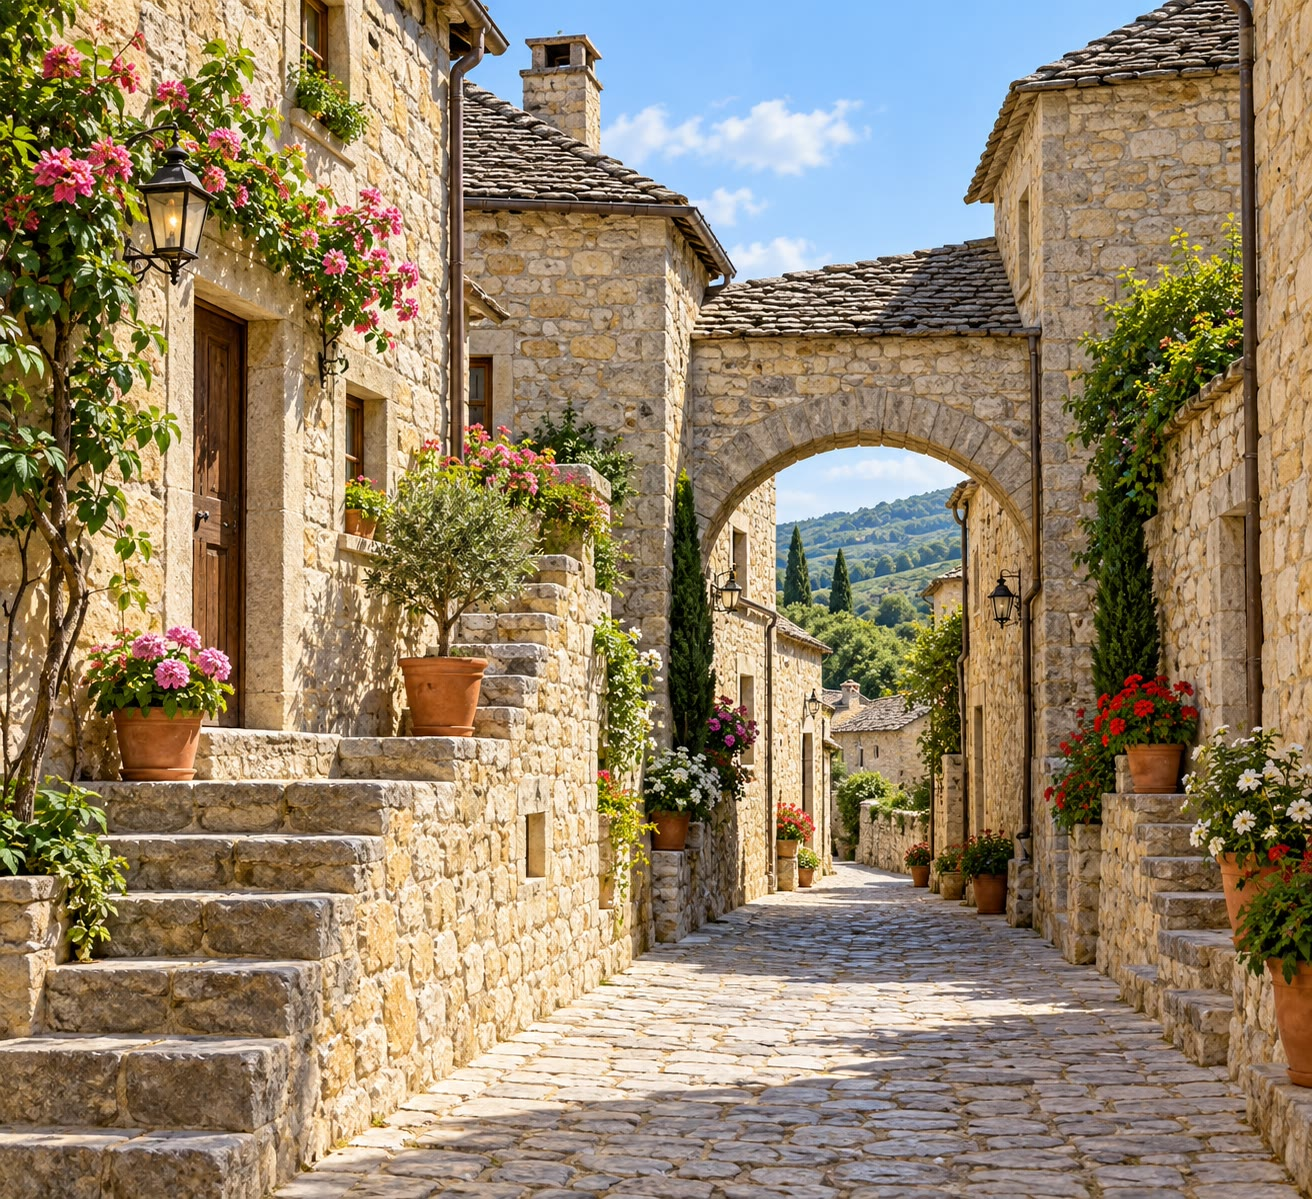
\includegraphics[width=0.6\linewidth]{images/book1/ai/g3-stone-village.jpg}

{\small قرية قديمة بُنيت كلها بحجر \omterm{def:g1:landscapes-around-us:landform}{التلة} القريبة.}
\end{omfigure}

واليوم نبني أيضًا بالطوب والخرسانة والزجاج. لكن الطوب يُصنع من الطين
المشوي، والخرسانة من \omterm{def:g3:stones-pebbles-sand:sand}{الرمل} \omterm{def:g3:stones-pebbles-sand:pebble}{والحصباء} والإسمنت، والزجاج من \omterm{def:g3:stones-pebbles-sand:sand}{الرمل}: وكلها تأتي
هي أيضًا من \omterm{def:g3:stones-pebbles-sand:rock}{صخور} الأرض.

\section{تمارين}

\begin{exercise}[$\star$]\label{exo:g3:stones-pebbles-sand:1}
ما \omterm{def:g3:stones-pebbles-sand:rock}{الصخر الأساسي}؟ وأين نستطيع أن نراه دون أن نحفر؟
\end{exercise}

\begin{exercise}[$\star$]\label{exo:g3:stones-pebbles-sand:2}
رتّب بحسب الحجم، من الأصغر إلى الأكبر: \omterm{def:g3:stones-pebbles-sand:pebble}{حصاة}، \omterm{def:g3:stones-pebbles-sand:sand}{وحل}،
جلمود، \omterm{def:g3:stones-pebbles-sand:sand}{رمل}.
\end{exercise}

\begin{exercise}[$\star$]\label{exo:g3:stones-pebbles-sand:3}
قطر حبة 1 مليمتر. أهي \omterm{def:g3:stones-pebbles-sand:sand}{رمل} أم \omterm{def:g3:stones-pebbles-sand:pebble}{حصباء}؟ وقطر حبة أخرى
3 مليمترات: \omterm{def:g3:stones-pebbles-sand:sand}{رمل} أم \omterm{def:g3:stones-pebbles-sand:pebble}{حصباء}؟
\end{exercise}

\begin{exercise}[$\star$]\label{exo:g3:stones-pebbles-sand:4}
طبيعي أم من صنع الإنسان؟ \omterm{def:g3:stones-pebbles-sand:pebble}{حصاة}؛ طوبة؛ كتلة غرانيت؛ لوح
زجاج؛ \omterm{def:g3:stones-pebbles-sand:sand}{رمل} على شاطئ.
\end{exercise}

\begin{exercise}[$\star$]\label{exo:g3:stones-pebbles-sand:5}
لماذا لا تكون \omterm{def:g3:stones-pebbles-sand:pebble}{لحصاة} \omterm{def:g1:landscapes-around-us:water}{النهر} زوايا حادة؟
\end{exercise}

\begin{exercise}[$\star$]\label{exo:g3:stones-pebbles-sand:6}
سمِّ حجرين من \omterm{def:g3:stones-pebbles-sand:building-stone}{حجارة البناء} وقل فيمَ يُستعمل كل منهما في صور
هذا الفصل.
\end{exercise}

\begin{exercise}[$\star\star$]\label{exo:g3:stones-pebbles-sand:7}
يجد توم حجرين من \omterm{def:g3:stones-pebbles-sand:rock}{الصخر} نفسه: أحدهما حاد، والآخر مستدير.
أيهما سافر أبعد؟ اشرح.
\end{exercise}

\begin{exercise}[$\star\star$]\label{exo:g3:stones-pebbles-sand:8}
في رسم أحجام الحبيبات، كم سنتيمترًا طول أكبر \omterm{def:g3:stones-pebbles-sand:pebble}{حصاة}؟
وكم حبة \omterm{def:g3:stones-pebbles-sand:sand}{رمل} قطرها 2 مليمتر تتسع جنبًا إلى جنب على طول 1
سنتيمتر؟
\end{exercise}

\begin{exercise}[$\star\star$]\label{exo:g3:stones-pebbles-sand:9}
أين تتوقع أن تجد \omterm{def:g3:stones-pebbles-sand:sand}{الوحل}: في جدول جبلي سريع أم في بركة
هادئة؟ لماذا؟
\end{exercise}

\begin{exercise}[$\star\star$]\label{exo:g3:stones-pebbles-sand:10}
الطوب والخرسانة والزجاج يصنعها الناس. فلماذا نستطيع مع ذلك أن نقول إنها
تأتي من \omterm{def:g3:stones-pebbles-sand:rock}{صخور} الأرض؟
\end{exercise}
